\section{Your Task}

As stated previously, your task for this assignment is to write a shell script,
or more specifically, a \Bash{} script. You will use this script to
produce plots of a provided \C{} program. The provided program can be
found in the resources repository.

All the program does is print the Collatz sequence starting from some positive
integer $n$. For those unacquainted with Collatz sequences, or more broadly, the
\emph{Collatz conjecture}, the setup is as follows: We will create a sequence of
integers $S$ starting with some positive integer $n$. That is, $S_1 = n$. The
next term of the sequence is based on the previous term of the sequence. In this
case, $S_2$, the second term of the sequence, is based on $S_1$, the first term
of the sequence. For any $S_{k+1}$ where $k > 0$, the following relation holds:
$$
\begin{aligned}
S_{k+1} =
  \begin{cases}
    1+3S_k  &\text{if $S_k$ is odd} \\
    \frac{1}{2}S_k &\text{if $S_k$ is even}
  \end{cases}
\end{aligned}
$$
The conjecture itself is that any sequence following this relation always ends
with the last term being $1$, no matter what $n$ was used to start the sequence
with. This has never been proved. If you do find a sequence that does not terminate, then you \emph{may be famous}, but more likely \emph{your code has a bug}.
According to Paul Erd\H{o}s, ``Mathematics may
not be ready for such problems.''

Using the provided Collatz program, you are expected to:
\begin{enumerate}
  \item Familiarize yourself with the syntax of \C{}.
  \item Understand what the provided program is doing. You will want to attend
    section for any parts you are unsure about.
  \item Produce interesting plots using the Collatz sequences produced by the
    provided program. You should use \texttt{gnuplot} to produce these plots,
    and everything should be automated by means of a \Bash{} script.
\end{enumerate}

Refer to Figures \ref{figure:collatz-length}, \ref{figure:collatz-maxval}, and
\ref{figure:collatz-hist} for example plots that were created using the provided
program. Now that you know your task, we will now give a brief overview on
\Bash{} scripting.

\begin{figure}[htb]
  \centering
  % GNUPLOT: LaTeX picture with Postscript
\begingroup
  \makeatletter
  \providecommand\color[2][]{%
    \GenericError{(gnuplot) \space\space\space\@spaces}{%
      Package color not loaded in conjunction with
      terminal option `colourtext'%
    }{See the gnuplot documentation for explanation.%
    }{Either use 'blacktext' in gnuplot or load the package
      color.sty in LaTeX.}%
    \renewcommand\color[2][]{}%
  }%
  \providecommand\includegraphics[2][]{%
    \GenericError{(gnuplot) \space\space\space\@spaces}{%
      Package graphicx or graphics not loaded%
    }{See the gnuplot documentation for explanation.%
    }{The gnuplot epslatex terminal needs graphicx.sty or graphics.sty.}%
    \renewcommand\includegraphics[2][]{}%
  }%
  \providecommand\rotatebox[2]{#2}%
  \@ifundefined{ifGPcolor}{%
    \newif\ifGPcolor
    \GPcolorfalse
  }{}%
  \@ifundefined{ifGPblacktext}{%
    \newif\ifGPblacktext
    \GPblacktexttrue
  }{}%
  % define a \g@addto@macro without @ in the name:
  \let\gplgaddtomacro\g@addto@macro
  % define empty templates for all commands taking text:
  \gdef\gplbacktext{}%
  \gdef\gplfronttext{}%
  \makeatother
  \ifGPblacktext
    % no textcolor at all
    \def\colorrgb#1{}%
    \def\colorgray#1{}%
  \else
    % gray or color?
    \ifGPcolor
      \def\colorrgb#1{\color[rgb]{#1}}%
      \def\colorgray#1{\color[gray]{#1}}%
      \expandafter\def\csname LTw\endcsname{\color{white}}%
      \expandafter\def\csname LTb\endcsname{\color{black}}%
      \expandafter\def\csname LTa\endcsname{\color{black}}%
      \expandafter\def\csname LT0\endcsname{\color[rgb]{1,0,0}}%
      \expandafter\def\csname LT1\endcsname{\color[rgb]{0,1,0}}%
      \expandafter\def\csname LT2\endcsname{\color[rgb]{0,0,1}}%
      \expandafter\def\csname LT3\endcsname{\color[rgb]{1,0,1}}%
      \expandafter\def\csname LT4\endcsname{\color[rgb]{0,1,1}}%
      \expandafter\def\csname LT5\endcsname{\color[rgb]{1,1,0}}%
      \expandafter\def\csname LT6\endcsname{\color[rgb]{0,0,0}}%
      \expandafter\def\csname LT7\endcsname{\color[rgb]{1,0.3,0}}%
      \expandafter\def\csname LT8\endcsname{\color[rgb]{0.5,0.5,0.5}}%
    \else
      % gray
      \def\colorrgb#1{\color{black}}%
      \def\colorgray#1{\color[gray]{#1}}%
      \expandafter\def\csname LTw\endcsname{\color{white}}%
      \expandafter\def\csname LTb\endcsname{\color{black}}%
      \expandafter\def\csname LTa\endcsname{\color{black}}%
      \expandafter\def\csname LT0\endcsname{\color{black}}%
      \expandafter\def\csname LT1\endcsname{\color{black}}%
      \expandafter\def\csname LT2\endcsname{\color{black}}%
      \expandafter\def\csname LT3\endcsname{\color{black}}%
      \expandafter\def\csname LT4\endcsname{\color{black}}%
      \expandafter\def\csname LT5\endcsname{\color{black}}%
      \expandafter\def\csname LT6\endcsname{\color{black}}%
      \expandafter\def\csname LT7\endcsname{\color{black}}%
      \expandafter\def\csname LT8\endcsname{\color{black}}%
    \fi
  \fi
    \setlength{\unitlength}{0.0500bp}%
    \ifx\gptboxheight\undefined%
      \newlength{\gptboxheight}%
      \newlength{\gptboxwidth}%
      \newsavebox{\gptboxtext}%
    \fi%
    \setlength{\fboxrule}{0.5pt}%
    \setlength{\fboxsep}{1pt}%
    \definecolor{tbcol}{rgb}{1,1,1}%
\begin{picture}(7200.00,5040.00)%
    \gplgaddtomacro\gplbacktext{%
      \csname LTb\endcsname%%
      \put(814,704){\makebox(0,0)[r]{\strut{}$0$}}%
      \put(814,1317){\makebox(0,0)[r]{\strut{}$50$}}%
      \put(814,1929){\makebox(0,0)[r]{\strut{}$100$}}%
      \put(814,2542){\makebox(0,0)[r]{\strut{}$150$}}%
      \put(814,3154){\makebox(0,0)[r]{\strut{}$200$}}%
      \put(814,3767){\makebox(0,0)[r]{\strut{}$250$}}%
      \put(814,4379){\makebox(0,0)[r]{\strut{}$300$}}%
      \put(946,484){\makebox(0,0){\strut{}$0$}}%
      \put(1532,484){\makebox(0,0){\strut{}$1000$}}%
      \put(2117,484){\makebox(0,0){\strut{}$2000$}}%
      \put(2703,484){\makebox(0,0){\strut{}$3000$}}%
      \put(3289,484){\makebox(0,0){\strut{}$4000$}}%
      \put(3875,484){\makebox(0,0){\strut{}$5000$}}%
      \put(4460,484){\makebox(0,0){\strut{}$6000$}}%
      \put(5046,484){\makebox(0,0){\strut{}$7000$}}%
      \put(5632,484){\makebox(0,0){\strut{}$8000$}}%
      \put(6217,484){\makebox(0,0){\strut{}$9000$}}%
      \put(6803,484){\makebox(0,0){\strut{}$10000$}}%
    }%
    \gplgaddtomacro\gplfronttext{%
      \csname LTb\endcsname%%
      \put(209,2541){\rotatebox{-270}{\makebox(0,0){\strut{}length}}}%
      \put(3874,154){\makebox(0,0){\strut{}$n$}}%
      \csname LTb\endcsname%%
      \put(3874,4709){\makebox(0,0){\strut{}Collatz Sequence Lengths}}%
    }%
    \gplbacktext
    \put(0,0){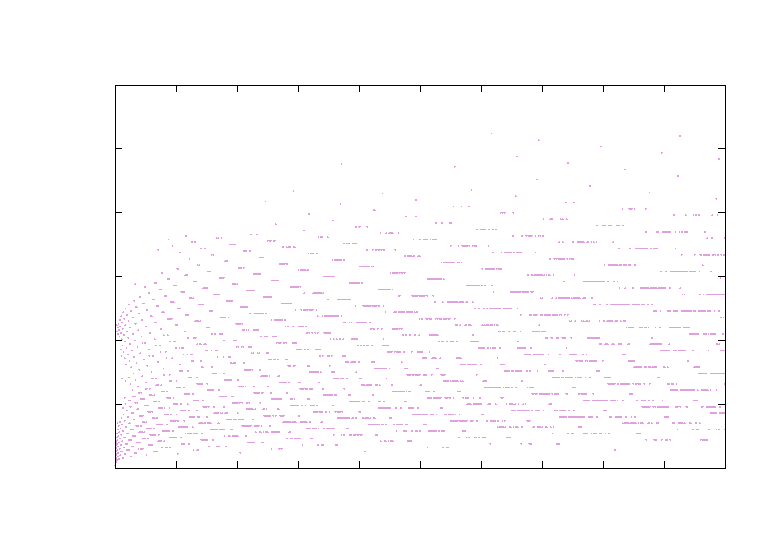
\includegraphics[width={360.00bp},height={252.00bp}]{figures/collatz_length}}%
    \gplfronttext
  \end{picture}%
\endgroup

  \caption{\label{figure:collatz-length}
    The length of Collatz sequences starting from $n \in \{\,2,\dots,10000\,\}$.
  }
\end{figure}

\begin{figure}[bth]
  \centering
  % GNUPLOT: LaTeX picture with Postscript
\begingroup
  \makeatletter
  \providecommand\color[2][]{%
    \GenericError{(gnuplot) \space\space\space\@spaces}{%
      Package color not loaded in conjunction with
      terminal option `colourtext'%
    }{See the gnuplot documentation for explanation.%
    }{Either use 'blacktext' in gnuplot or load the package
      color.sty in LaTeX.}%
    \renewcommand\color[2][]{}%
  }%
  \providecommand\includegraphics[2][]{%
    \GenericError{(gnuplot) \space\space\space\@spaces}{%
      Package graphicx or graphics not loaded%
    }{See the gnuplot documentation for explanation.%
    }{The gnuplot epslatex terminal needs graphicx.sty or graphics.sty.}%
    \renewcommand\includegraphics[2][]{}%
  }%
  \providecommand\rotatebox[2]{#2}%
  \@ifundefined{ifGPcolor}{%
    \newif\ifGPcolor
    \GPcolorfalse
  }{}%
  \@ifundefined{ifGPblacktext}{%
    \newif\ifGPblacktext
    \GPblacktexttrue
  }{}%
  % define a \g@addto@macro without @ in the name:
  \let\gplgaddtomacro\g@addto@macro
  % define empty templates for all commands taking text:
  \gdef\gplbacktext{}%
  \gdef\gplfronttext{}%
  \makeatother
  \ifGPblacktext
    % no textcolor at all
    \def\colorrgb#1{}%
    \def\colorgray#1{}%
  \else
    % gray or color?
    \ifGPcolor
      \def\colorrgb#1{\color[rgb]{#1}}%
      \def\colorgray#1{\color[gray]{#1}}%
      \expandafter\def\csname LTw\endcsname{\color{white}}%
      \expandafter\def\csname LTb\endcsname{\color{black}}%
      \expandafter\def\csname LTa\endcsname{\color{black}}%
      \expandafter\def\csname LT0\endcsname{\color[rgb]{1,0,0}}%
      \expandafter\def\csname LT1\endcsname{\color[rgb]{0,1,0}}%
      \expandafter\def\csname LT2\endcsname{\color[rgb]{0,0,1}}%
      \expandafter\def\csname LT3\endcsname{\color[rgb]{1,0,1}}%
      \expandafter\def\csname LT4\endcsname{\color[rgb]{0,1,1}}%
      \expandafter\def\csname LT5\endcsname{\color[rgb]{1,1,0}}%
      \expandafter\def\csname LT6\endcsname{\color[rgb]{0,0,0}}%
      \expandafter\def\csname LT7\endcsname{\color[rgb]{1,0.3,0}}%
      \expandafter\def\csname LT8\endcsname{\color[rgb]{0.5,0.5,0.5}}%
    \else
      % gray
      \def\colorrgb#1{\color{black}}%
      \def\colorgray#1{\color[gray]{#1}}%
      \expandafter\def\csname LTw\endcsname{\color{white}}%
      \expandafter\def\csname LTb\endcsname{\color{black}}%
      \expandafter\def\csname LTa\endcsname{\color{black}}%
      \expandafter\def\csname LT0\endcsname{\color{black}}%
      \expandafter\def\csname LT1\endcsname{\color{black}}%
      \expandafter\def\csname LT2\endcsname{\color{black}}%
      \expandafter\def\csname LT3\endcsname{\color{black}}%
      \expandafter\def\csname LT4\endcsname{\color{black}}%
      \expandafter\def\csname LT5\endcsname{\color{black}}%
      \expandafter\def\csname LT6\endcsname{\color{black}}%
      \expandafter\def\csname LT7\endcsname{\color{black}}%
      \expandafter\def\csname LT8\endcsname{\color{black}}%
    \fi
  \fi
    \setlength{\unitlength}{0.0500bp}%
    \ifx\gptboxheight\undefined%
      \newlength{\gptboxheight}%
      \newlength{\gptboxwidth}%
      \newsavebox{\gptboxtext}%
    \fi%
    \setlength{\fboxrule}{0.5pt}%
    \setlength{\fboxsep}{1pt}%
    \definecolor{tbcol}{rgb}{1,1,1}%
\begin{picture}(7200.00,5040.00)%
    \gplgaddtomacro\gplbacktext{%
      \csname LTb\endcsname%%
      \put(1210,704){\makebox(0,0)[r]{\strut{}$0$}}%
      \put(1210,1439){\makebox(0,0)[r]{\strut{}$20000$}}%
      \put(1210,2174){\makebox(0,0)[r]{\strut{}$40000$}}%
      \put(1210,2909){\makebox(0,0)[r]{\strut{}$60000$}}%
      \put(1210,3644){\makebox(0,0)[r]{\strut{}$80000$}}%
      \put(1210,4379){\makebox(0,0)[r]{\strut{}$100000$}}%
      \put(1342,484){\makebox(0,0){\strut{}$0$}}%
      \put(1888,484){\makebox(0,0){\strut{}$1000$}}%
      \put(2434,484){\makebox(0,0){\strut{}$2000$}}%
      \put(2980,484){\makebox(0,0){\strut{}$3000$}}%
      \put(3526,484){\makebox(0,0){\strut{}$4000$}}%
      \put(4073,484){\makebox(0,0){\strut{}$5000$}}%
      \put(4619,484){\makebox(0,0){\strut{}$6000$}}%
      \put(5165,484){\makebox(0,0){\strut{}$7000$}}%
      \put(5711,484){\makebox(0,0){\strut{}$8000$}}%
      \put(6257,484){\makebox(0,0){\strut{}$9000$}}%
      \put(6803,484){\makebox(0,0){\strut{}$10000$}}%
    }%
    \gplgaddtomacro\gplfronttext{%
      \csname LTb\endcsname%%
      \put(209,2541){\rotatebox{-270}{\makebox(0,0){\strut{}value}}}%
      \put(4072,154){\makebox(0,0){\strut{}$n$}}%
      \csname LTb\endcsname%%
      \put(4072,4709){\makebox(0,0){\strut{}Maximum Collatz Sequence Value}}%
    }%
    \gplbacktext
    \put(0,0){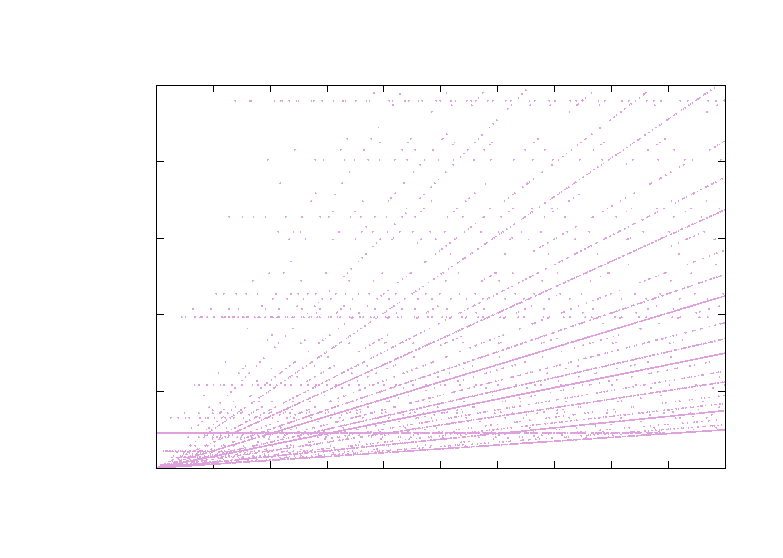
\includegraphics[width={360.00bp},height={252.00bp}]{figures/collatz_maxval}}%
    \gplfronttext
  \end{picture}%
\endgroup

  \caption{\label{figure:collatz-maxval}
    The maximum values for Collatz sequences starting from $n \in
    \{\,2,\dots,10000\,\}$.
  }
\end{figure}

\begin{figure}[bth]
  \centering
  % GNUPLOT: LaTeX picture with Postscript
\begingroup
  \makeatletter
  \providecommand\color[2][]{%
    \GenericError{(gnuplot) \space\space\space\@spaces}{%
      Package color not loaded in conjunction with
      terminal option `colourtext'%
    }{See the gnuplot documentation for explanation.%
    }{Either use 'blacktext' in gnuplot or load the package
      color.sty in LaTeX.}%
    \renewcommand\color[2][]{}%
  }%
  \providecommand\includegraphics[2][]{%
    \GenericError{(gnuplot) \space\space\space\@spaces}{%
      Package graphicx or graphics not loaded%
    }{See the gnuplot documentation for explanation.%
    }{The gnuplot epslatex terminal needs graphicx.sty or graphics.sty.}%
    \renewcommand\includegraphics[2][]{}%
  }%
  \providecommand\rotatebox[2]{#2}%
  \@ifundefined{ifGPcolor}{%
    \newif\ifGPcolor
    \GPcolorfalse
  }{}%
  \@ifundefined{ifGPblacktext}{%
    \newif\ifGPblacktext
    \GPblacktexttrue
  }{}%
  % define a \g@addto@macro without @ in the name:
  \let\gplgaddtomacro\g@addto@macro
  % define empty templates for all commands taking text:
  \gdef\gplbacktext{}%
  \gdef\gplfronttext{}%
  \makeatother
  \ifGPblacktext
    % no textcolor at all
    \def\colorrgb#1{}%
    \def\colorgray#1{}%
  \else
    % gray or color?
    \ifGPcolor
      \def\colorrgb#1{\color[rgb]{#1}}%
      \def\colorgray#1{\color[gray]{#1}}%
      \expandafter\def\csname LTw\endcsname{\color{white}}%
      \expandafter\def\csname LTb\endcsname{\color{black}}%
      \expandafter\def\csname LTa\endcsname{\color{black}}%
      \expandafter\def\csname LT0\endcsname{\color[rgb]{1,0,0}}%
      \expandafter\def\csname LT1\endcsname{\color[rgb]{0,1,0}}%
      \expandafter\def\csname LT2\endcsname{\color[rgb]{0,0,1}}%
      \expandafter\def\csname LT3\endcsname{\color[rgb]{1,0,1}}%
      \expandafter\def\csname LT4\endcsname{\color[rgb]{0,1,1}}%
      \expandafter\def\csname LT5\endcsname{\color[rgb]{1,1,0}}%
      \expandafter\def\csname LT6\endcsname{\color[rgb]{0,0,0}}%
      \expandafter\def\csname LT7\endcsname{\color[rgb]{1,0.3,0}}%
      \expandafter\def\csname LT8\endcsname{\color[rgb]{0.5,0.5,0.5}}%
    \else
      % gray
      \def\colorrgb#1{\color{black}}%
      \def\colorgray#1{\color[gray]{#1}}%
      \expandafter\def\csname LTw\endcsname{\color{white}}%
      \expandafter\def\csname LTb\endcsname{\color{black}}%
      \expandafter\def\csname LTa\endcsname{\color{black}}%
      \expandafter\def\csname LT0\endcsname{\color{black}}%
      \expandafter\def\csname LT1\endcsname{\color{black}}%
      \expandafter\def\csname LT2\endcsname{\color{black}}%
      \expandafter\def\csname LT3\endcsname{\color{black}}%
      \expandafter\def\csname LT4\endcsname{\color{black}}%
      \expandafter\def\csname LT5\endcsname{\color{black}}%
      \expandafter\def\csname LT6\endcsname{\color{black}}%
      \expandafter\def\csname LT7\endcsname{\color{black}}%
      \expandafter\def\csname LT8\endcsname{\color{black}}%
    \fi
  \fi
    \setlength{\unitlength}{0.0500bp}%
    \ifx\gptboxheight\undefined%
      \newlength{\gptboxheight}%
      \newlength{\gptboxwidth}%
      \newsavebox{\gptboxtext}%
    \fi%
    \setlength{\fboxrule}{0.5pt}%
    \setlength{\fboxsep}{1pt}%
    \definecolor{tbcol}{rgb}{1,1,1}%
\begin{picture}(7200.00,5040.00)%
    \gplgaddtomacro\gplbacktext{%
      \csname LTb\endcsname%%
      \put(814,704){\makebox(0,0)[r]{\strut{}$0$}}%
      \put(814,1072){\makebox(0,0)[r]{\strut{}$20$}}%
      \put(814,1439){\makebox(0,0)[r]{\strut{}$40$}}%
      \put(814,1807){\makebox(0,0)[r]{\strut{}$60$}}%
      \put(814,2174){\makebox(0,0)[r]{\strut{}$80$}}%
      \put(814,2542){\makebox(0,0)[r]{\strut{}$100$}}%
      \put(814,2909){\makebox(0,0)[r]{\strut{}$120$}}%
      \put(814,3277){\makebox(0,0)[r]{\strut{}$140$}}%
      \put(814,3644){\makebox(0,0)[r]{\strut{}$160$}}%
      \put(814,4012){\makebox(0,0)[r]{\strut{}$180$}}%
      \put(814,4379){\makebox(0,0)[r]{\strut{}$200$}}%
      \put(946,484){\makebox(0,0){\strut{}$0$}}%
      \put(1597,484){\makebox(0,0){\strut{}$25$}}%
      \put(2248,484){\makebox(0,0){\strut{}$50$}}%
      \put(2898,484){\makebox(0,0){\strut{}$75$}}%
      \put(3549,484){\makebox(0,0){\strut{}$100$}}%
      \put(4200,484){\makebox(0,0){\strut{}$125$}}%
      \put(4851,484){\makebox(0,0){\strut{}$150$}}%
      \put(5501,484){\makebox(0,0){\strut{}$175$}}%
      \put(6152,484){\makebox(0,0){\strut{}$200$}}%
      \put(6803,484){\makebox(0,0){\strut{}$225$}}%
    }%
    \gplgaddtomacro\gplfronttext{%
      \csname LTb\endcsname%%
      \put(209,2541){\rotatebox{-270}{\makebox(0,0){\strut{}frequency}}}%
      \put(3874,154){\makebox(0,0){\strut{}length}}%
      \csname LTb\endcsname%%
      \put(3874,4709){\makebox(0,0){\strut{}Collatz Sequence Length Histogram}}%
    }%
    \gplbacktext
    \put(0,0){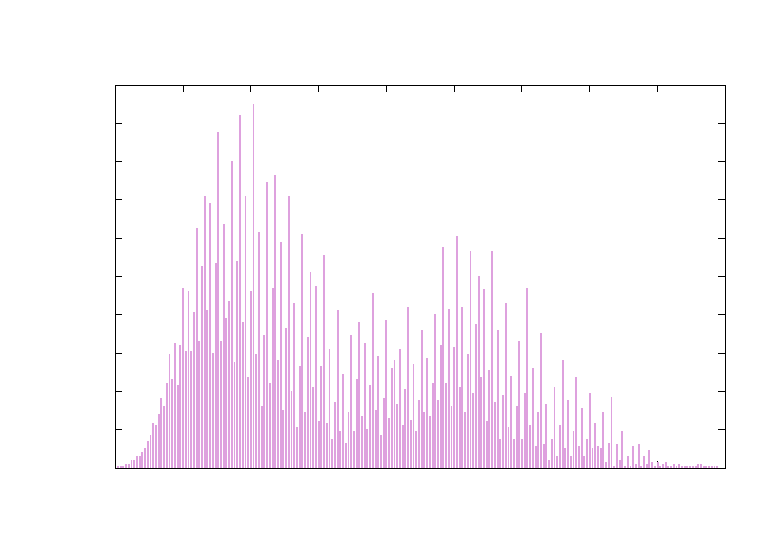
\includegraphics[width={360.00bp},height={252.00bp}]{figures/collatz_hist}}%
    \gplfronttext
  \end{picture}%
\endgroup

  \caption{\label{figure:collatz-hist}
    A histogram of Collatz sequence lengths starting from $n \in
    \{\,2,\dots,10000\,\}$.
  }
\end{figure}
